\documentclass{beamer}
\usepackage[ngerman]{babel}
\usepackage[utf8]{inputenc}
\usepackage{graphicx}
\usepackage{amssymb} 
\usepackage{amsmath}

\usepackage{hyperref}

\usetheme{Warsaw}
\usecolortheme{default}


\author{Richard Feistenauer}
\title{12. GBI-Tutorium von Tutorium Nr.31}
\date{30.Januar 2015}

\begin{document}

\begin {frame}
	\titlepage
\end {frame}

\begin {frame}
	\frametitle {Inhaltsverzeichnis}
	\tableofcontents
\end {frame}

\section{Strukturelle Induktion}

\begin{frame}
	\frametitle{die sogenannte strukturelle Induktion}
	\begin{block}{Definition}
		Die strukturelle Induktion ist eine verallgemeinerte vollständige Induktion.
		\begin{itemize}
			\item Sie besitzt wie auch die vollständige Induktion IA,IV,IS.
			\item IA: man zeigt die Behauptung für alle atomar
			\item IS: man zeigt das die atomaren Behauptungen auch für die allgemeine Formel gelten.
			\item Sie wird verwendet um z. B. eine Abhängigkeit von Elementen von einer Menge zu überprüfen.
		\end{itemize}
	\end{block}
\end{frame}

\begin{frame}
	\frametitle{Beispiel zur s. Induktion}
	\begin{block}{Beispiel Aufgabe}
		Die Sprache L $\subseteq$ \{a,b\}$^\ast$ sei wie folgt definiert:
		\begin{itemize}
			\item $\epsilon \in$ L 
			\item $\forall w_1, w_2 \in L: aw_1bw_2 \in L \wedge bw_1aw_2 \in L$
			\item Keine anderen Wörter liegen in L.
		\end{itemize}
		Zeigen sie durch strukturelle Induktion, dass jedes Wort w $\in$ L ebenso viele a wie b enthält. (Schreibweise für Anzahl der a in w : $N_a(w)$)
	\end{block}
\end{frame}

\section{Partiell definierte Funktionen}

\begin{frame}
	\frametitle{Partiell definierte Funktionen}
	\begin{block}{Einschub: Partiell definierte Funktionen}
		\begin{itemize}
			\item Bisher bekannt: (Total definierte) Funktionen
			\item Diese entsprechen linkstotalen rechtseindeutigen Relationen\\ (Jedem Element aus der Definitionsmenge wird genau 1 Element aus der Zielmenge zugewiesen).
			\item Jetzt: Partiell definierte Funktionen
			\item Diese entsprechen rechtseindeutigen Relationen\\ (Manchen Elementen aus der Definitionsmenge wird genau 1 Element aus der Zielmenge zugewiesen).\\ $\Rightarrow$ Für manche Werte ist die partiell definierte Funktion undefiniert.
		\end{itemize}
	\end{block}
\end{frame}

\section{Turingmaschinen}
\begin{frame}
	\frametitle{Definition der Turingmaschine}
	\begin{block}{T = \{Z,z$_0$,X,f,g,m\}}
		\begin{itemize}
			\item eine Zustandsmenge Z
			\item einen Anfangszustand z$_0 \in$ Z
			\item ein Bandalphabet X\\ (meist mit Blanksymbol $\Box$) 
			\item eine partielle Zustandsüberführungsfunktion\\
			f : Z x X $\rightarrow$ Z
			\item eine partielle Ausgabefunktion\\
			g : Z x X $\rightarrow$ X
			\item eine partielle Bewegungsfunktion\\
			m : Z x X $\rightarrow$ \{-1,0,1\} oder \{L,0,R\}
			\item f,g,m für die gleichen Paare\\
			(z,x) $\in$ Z x X definiert bzw. nicht definiert
		\end{itemize}	
	\end{block}		
\end{frame}

\begin{frame}
	\frametitle{Erklärung zur Turingmaschine}
	\begin{block}{Was ist eine Turingmaschine}
		Eine Turingmaschine ist eine Maschine, die ein Eingabewort auf einem Band lesen kann, dieses Band überschreiben kann, und somit verschiedene Arbeitsaufträge machen kann.
		Bestandteile:
		\begin{itemize}
			\item Arbeitsband (hier steht Ein- und Ausgabe)
			\item ein Kopf der lesen, schreiben und bewegt werden kann, von Buchstabe zu Buchstabe.
		\end{itemize}
		eine Turingmaschine hält an wenn für eine Eingabe kein Übergang definiert ist.
	\end{block}
\end{frame}

\begin{frame}
	\begin{block}{Beispiel}
		\begin{figure}[H]
  			\centering
  			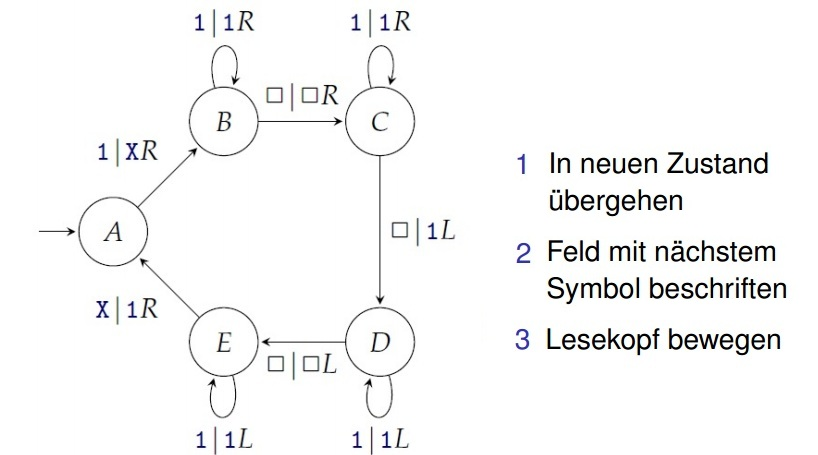
\includegraphics[width=\textwidth]{Turing1.jpg}
  			\caption{Turingmaschine}
  			\label{Turingmaschine}
		\end{figure}
	\end{block}
\end{frame}

\begin{frame}
	\frametitle{Tabellen Repräsentation}
	\begin{block}{Turingmaschine als Tabelle}
		\begin{tabular}{|c||c|c|c|c|c|}
			\hline
			  & A & B & C & D & E \\
			\hline
			\hline
			$\Box$ & & C,$\Box$,R & D,1,L & E,$\Box$,L & \\	
			\hline
			1 & B,X,R & B,1,R & C,1,R & D,1,L & E,1,L\\
			\hline
			X & & & & & A,1,R\\	
			\hline
		\end{tabular}
	\end{block}
\end{frame}

\section{Berechnungskomplexität}
\begin{frame}
	\frametitle{Berechnungen}
	\begin{block}{Berechnungszeit}
		Wie lang kann so eine Turingmaschine denn schätzungsweise für eine Berechnung maximal brauchen. (in Abhängigkeit zur Länge des Eingabewortes n)\\
		\bigskip
		\pause
		unendlich, da eine Turingmaschine nicht anhalten muss.\\
		
		In diesem Abschnitt gehen wir jetzt aber von Turingmaschinen aus die für jede Eingabe halten.
	\end{block}
\end{frame}

\begin{frame}
	\frametitle{Berechnungskomplexität}
	\begin{block}{Funktionen}
		zur Berechnung der Komplexität einer Turingmaschine gibt es die Funktionen 	
		\begin{itemize}
			\item für die Zeitkomplexität\\
			\begin{itemize}
				\item time$_T$(w)
				\item Time$_T$(n)
			\end{itemize}
			\item für die Raumkomplexität\\
			\begin{itemize}
				\item space$_T$(w)
				\item Space$_T$(n)			
			\end{itemize}
		\end{itemize}	
		
		Wobei üblicherweise die Abbildung\\
		Time$_T$ die Zeitkomplexität der Turingmaschine T heißt und\\
		Space$_T$ die Raumkomplexität der Turingmaschine T.
	\end{block}
\end{frame}

\begin{frame}
	\frametitle{weiteres zur Berechnungskomplexität}
	\begin{block}{Infos}
		Man sagt, dass die Zeit- oder Raumkomplexität einer Turingmaschine polynomiell ist, wenn ein Polynom p(n) existiert, so dass Time$_T \in$ O(p(n)) bzw. Space$_T \in$ O(p(n)) ist.\\
		auserdem gilt: space(w) $\leq$ max(|w|, 1 + time(w)).
	\end{block}
\end{frame}

\begin{frame}
\frametitle{Ende}
	\begin{center}
		Noch Fragen?
	\end{center}
\end{frame}

\begin{frame}
\frametitle{Unnützes Wissen}
	\begin{center}
		Los Angeles' vollständiger Name ist "El Pueblo de Nuestra Senora la Reina de los Angeles de Porciuncula" und kann auf 3,6\% seiner Länge zu "L. A." verkürzt werden.
	\end{center}
\end{frame}

\end{document}